\documentclass[../main.tex]{subfiles}

\begin{document}

\problem{2}

Consider the problem of two steady, uniform, and incompressible fluid jets colliding at right angles as shown to form a common jet at an angle \(\theta\). 
The pressure everywhere is \(p_{atm}\), and gravity/shear stress can be safely neglected. 
The control volume is given by the dashed lines.
Write out, simplify (stating your assumptions), and solve the continuity equation and relevant momentum equations. 
Find the angle \(\theta\) in terms of the flow properties \(u_1, \dot{m}_1, v_2, \ \textrm{and} \ \dot{m}_2\) of the two jets (where \(\dot{m}\) is the mass flowrate). 
State your assumptions.

\begin{figure}[ht]
    \centering
    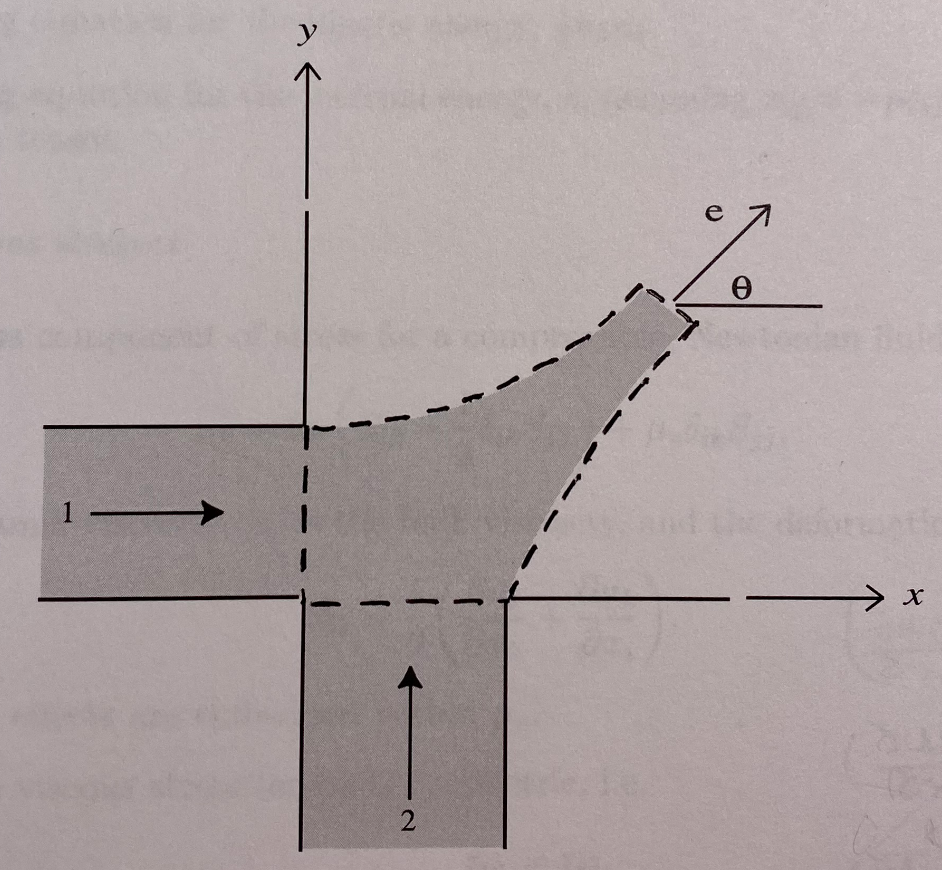
\includegraphics[scale=0.5]{images/problem2_diagram.png}
\end{figure}

\givens{}
\(u_1, \dot{m}_1, v_2, \dot{m}_2, \theta, p_{atm}\)

\assumptions{}
Steady, uniform, incompressible flow. 
Gravity and shear stress can be ignored. 
Pressure everywhere is $P_{atm}$.
Jets collide at a right angle.
All flow velocities are normal to inlets/outlets.

\solution{}
The full integral form of the conservation of mass equation is given by

\begin{equation*}
    \frac{\dd (m)_{sys}}{\dd t} = %
    \pdv{t} \int_{CV} \rho \dd \volume +%
    \int_{CS} \rho \left({\vec{V} \cdot \hat{\mathbf{n}}}\right) \dd A
    = 0
\end{equation*}

The assumption of steady flow removes the time-dependency of the continuity equation:

\begin{equation*}
    \cancelto{0}{\pdv{t} \int_{CV} \rho \dd \volume} +%
    \int_{CS} \rho \left({\vec{V} \cdot \hat{\mathbf{n}}}\right) \dd A
    = 0
\end{equation*}

\begin{equation*}
    \int_{CS} \rho \left({\vec{V} \cdot \hat{\mathbf{n}}}\right) \dd A
    = 0
\end{equation*}

The assumption of uniform flow removes the spatial dependence of the integrand:

\begin{equation*}
    \rho \left({\vec{V} \cdot \hat{\mathbf{n}}}\right) \int_{CS} \dd A
    = 0
\end{equation*}

This results in the following expression evaluated at every CS:

\begin{equation*}
    \left. \rho \left({\vec{V} \cdot \hat{\mathbf{n}}}\right) A \right|_{CS}
    = 0
\end{equation*}

The assumption of incompressibility implies that $\rho$ is constant throughout the flow and the same at every CS, and can therefore be divided out.

\begin{equation*}
    \left. \left({\vec{V} \cdot \hat{\mathbf{n}}}\right) A \right|_{CS}
    = 0
\end{equation*}

Recalling that \(\left({\vec{V} \cdot \hat{\mathbf{n}}}\right)\) can be expressed as \({-\lvert{\vec{V}_n}\rvert}\) for influx and \({+\lvert{\vec{V}_n}\rvert}\) for outflux, we rewrite the simplified form of the continuity equation in terms of influx and outflux:

\begin{equation*}
    \sum_{outflux} {\lvert{\vec{V}_n}\rvert A} -%
    \sum_{influx}  {\lvert{\vec{V}_n}\rvert A} = 0
\end{equation*}

\begin{equation*}
    \sum_{outflux} {\lvert{\vec{V}_n}\rvert A} = %
    \sum_{influx}  {\lvert{\vec{V}_n}\rvert A}
\end{equation*}

The sum of all mass influx terms must be equal to the sum of all outflux terms to satisfy continuity.

Examining our problem, with inlet control surfaces 1 and 2 and outlet control surface $e$, we apply the simplified form of continuity to yield:

\[
    V_1 A_1 + V_2 A_2 = V_e A_e  
\]

where $V_e$ represents the velocity in the exit direction.

Multiplying through by density yields an expression in terms of mass flow rate:

\[
    \rho V_1 A_1 + \rho V_2 A_2 = \rho V_e A_e
\]

\[
    \dot{m}_1 + \dot{m}_2 = \dot{m}_e
\]

The full integral form of the conservation of momentum equation is given by

\begin{equation*}
    \frac{\dd (m\vec{V})_{sys}}{\dd t} = %
    \pdv{t} \int_{CV} \rho \vec{V} \dd \volume +%
    \int_{CS} \rho \vec{V} \left({\vec{V} \cdot \hat{\mathbf{n}}}\right) \dd A =%
    \sum{\vec{F}_{CV}}
\end{equation*}

The sum of forces acting on the CV, \(\sum{\vec{F}_{CV}}\), can be found by summing the surface forces and body forces acting on the system. 

\begin{equation*}
    \sum{\vec{F}_{CV}} =%
    \int_{CV} \rho \vec{\mathbf{f}} \dd \volume -
    \int_{CS} p \hat{\mathbf{n}} \dd A +
    \vec{F}_{viscous} +
    \sum \vec{R} 
\end{equation*}

\[
    \pdv{t} \int_{CV} \rho \vec{V} \dd \volume +%
    \int_{CS} \rho \vec{V} \left({\vec{V} \cdot \hat{\mathbf{n}}}\right) \dd A =%
    \int_{CV} \rho \vec{\mathbf{f}} \dd \volume -
    \int_{CS} p \hat{\mathbf{n}} \dd A +
    \vec{F}_{viscous} +
    \sum \vec{R} 
\]


\end{document}